%!TEX program = xelatex

\documentclass[compress]{beamer}
%--------------------------------------------------------------------------
% Common packages
%--------------------------------------------------------------------------
\usepackage[english]{babel}
\usepackage{pgfpages} % required for notes on second screen
\usepackage{graphicx}

\usepackage{multicol}

\usepackage{tabularx,ragged2e}
\usepackage{booktabs}
\usepackage{multirow}

\setlength{\emergencystretch}{3em}  % prevent overfull lines

\usetheme{hri}

\usepackage{tikz}
\usetikzlibrary{mindmap,backgrounds,positioning,patterns}

\graphicspath{{figs/}}

\title{ROCO318 \newline Mobile and humanoid robots}
\subtitle{Part 2 -- Sensors and perception}
\date{}
\author{Séverin Lemaignan}
\institute{Centre for Neural Systems and Robotics\\{\bf Plymouth University}}

\begin{document}

\licenseframe{github.com/severin-lemaignan/[REPO]}

\maketitle

\begin{frame}{Part 2 -- Sensors and perception}

For further reading see Part C from (Siciliano and Khatib, 2008) or
chapter 4 of (Siegwart and Nourbakhsh, 2004).

\end{frame}

\section{Sensor classification}\label{sensor-classification}

\begin{frame}{Sensor classification}

\textbf{Proprioceptive} sensors

\begin{itemize}

\item
  measure values internally to the system (robot),
\item
  \eg motor speed, wheel load, heading of the robot, battery status
\end{itemize}

\textbf{Exteroceptive} sensors

\begin{itemize}

\item
  information from the robots environment
\item
  distances to objects, intensity of the ambient light, unique features.
\end{itemize}

\textbf{Passive} sensors

\begin{itemize}

\item
  energy coming from the environment
\end{itemize}

\textbf{Active} sensors

\begin{itemize}

\item
  emit their proper energy and measure the reaction
\item
  better performance, but some influence on envrionment
\end{itemize}

\end{frame}

\begin{frame}{Examples of classification (1/2)}

\scriptsize

\begin{tabular}{@{}p{4cm}p{4cm}ll@{}}
\toprule
{\bf General classification}\newline(typical use)                                                                                  & \bf Sensor\newline Sensor system & PC or EC & A or P \\ \midrule
\multirow{3}{\linewidth}{{\it Tactile sensors} \newline \tiny detection of physical contact or closeness; security switches}               & Contact switches, bumpers                                      & EC       & P      \\
                                                                                                                                                         & Optical barriers                                               & EC       & A      \\
                                                                                                                                                         & Noncontact proximity sensors                                   & EC       & A      \\ \midrule
\multirow{7}{\linewidth}{{\it Wheel/motor sensors} \newline \tiny wheel/motor speed and position}                                          & Brush encoders                                                 & PC       & P      \\
                                                                                                                                                         & Potentiometers                                                 & PC       & P      \\
                                                                                                                                                         & Synchros, resolvers                                            & PC       & A      \\
                                                                                                                                                         & Optical encoders                                               & PC       & A      \\
                                                                                                                                                         & Magnetic encoders                                              &          & A      \\
                                                                                                                                                         & Inductive encoders                                             & PC       & A      \\
                                                                                                                                                         & Capacitive encoders                                            & PC       & A      \\ \midrule
\multirow{3}{\linewidth}{{\it Heading sensors}\newline \tiny orientation of the robot in relation to a fixed reference frame}             & Compass                                                        & EC       & P      \\
                                                                                                                                                         & Gyroscopes                                                     & PC       & P      \\
                                                                                                                                                         & Inclinometers                                                  & EC       & A/P    \\ \bottomrule
\end{tabular}

PC: proprioceptive; EC: exteroceptive; A: active; P: passive; A/P: active/passive
\end{frame}

\begin{frame}{Examples of classification (2/2)}

\scriptsize

\begin{tabular}{@{}p{4cm}p{4cm}ll@{}}
\toprule
{\bf General classification}\newline(typical use)                                                                                  & \bf Sensor\newline Sensor system & PC or EC & A or P \\ \midrule
\multirow{4}{\linewidth}{{\it Ground-based beacons}\newline\tiny localization in a fixed reference frame}                                & GPS                                                            & EC       & A      \\
                                                                                                                                                         & Active optical of RF beacons                                   & EC       & A      \\
                                                                                                                                                         & Active ultrasonic beacons                                      & EC       & A      \\
                                                                                                                                                         & Reflective beacons                                             & EC       & A      \\ \midrule


\multirow{5}{\linewidth}{{\it Active ranging}\newline\tiny reflectivity, time-of-flight, geometric triangulation}                        & Reflectivity sensors                                           & EC       & A      \\
                                                                                                                                                         & Ultrasonic sensor                                              & EC       & A      \\
                                                                                                                                                         & Laser range finder                                             & EC       & A      \\
                                                                                                                                                         & Optical triangulation (1D)                                     & EC       & A      \\
                                                                                                                                                         & Structured light (2D)                                          & EC       & A      \\ \midrule
\multirow{2}{\linewidth}{{\it Motion/speed sensors}\newline\tiny speed relative to fixed or moving objects}                              & Doppler radar                                                  & EC       & A      \\
                                                                                                                                                         & Doppler sound                                                  & EC       & A      \\ \midrule
\multirow{3}{\linewidth}{{\it Vision-based sensors}\newline \tiny visual ranging, whole image analysis, segmentation, object recognition} & CCD/CMOS camera(s)                                             & EC       & P      \\
                                                                                                                                                         & Visual ranging packages                                        &          &        \\
                                                                                                                                                         & Object tracking packages                                       &          &        \\ \bottomrule
\end{tabular}


\end{frame}

%%%%%%%%%%%%%%%%%%%%%%%%%%%%%%%%%%%%%%%%%%%%%%%%%%%%%%%%%%%%%%%%%%%%%%%%%%%%%%%%%
%%%%%%%%%%%%%%%%%%%%%%%%%%%%%%%%%%%%%%%%%%%%%%%%%%%%%%%%%%%%%%%%%%%%%%%%%%%%%%%%%
\section[Characterizing Performance]{Characterizing Sensor Performance}\label{characterizing-sensor-performance}

\begin{frame}{Basic sensor response ratings (1/2)}

\begin{itemize}
    \item {\bf Dynamic range}: ratio between lower and upper limits, sometimes expressed
    in decibels (dB, power)
\[
\bubblemark{decibel}10\cdot \log_{10}\frac{P_{upper}}{P_{lower}}
\]

\bubble<1>[30]{decibel}{Multiplied by 10 to make the number a bit larger. That's why it's called
\emph{deci}Bel.}

        \begin{itemize}
        
        \item<3->
        \eg current measurement from 1 milliamp to 30 amps
        \[
            \bubblemark{twenty}20\cdot\log_{10}\frac{I_{upper}}{I_{lower}}=20\cdot\log_{10}\frac{30A}{0.001A}=90dB
        \]
    \bubble<3>[30][0.7cm]{twenty}{20 instead of 10 because square of current or voltage is proportional to power.}

        \item<4->
        \eg voltage measurement from 1 millivolt to 20 volt
        \[
            20\cdot\log_{10}\frac{I_{upper}}{I_{lower}}=20\cdot\log_{10}\frac{20V}{0.001V}=86dB
        \]
        \end{itemize}

    \item<5-> {\bf Range}
        \begin{itemize}
        
        \item upper and lower limits
        \end{itemize}



\end{itemize}

\end{frame}

%%%%%%%%%%%%%%%%%%%%%%%%%%%%%%%%%%%%%%%%%%%%%%%%%%%%%%%%%%%%%%

\begin{frame}{Basic sensor response ratings (2/2)}

    \begin{itemize}
        \item {\bf Resolution}
            \begin{itemize}
                \item minimum difference between two values
                \item usually: lower limit of dynamic range = resolution
                \item for digital sensors it is usually the A/D resolution,\\ \eg $ 5V / 255 $ (8 bit) 

            \end{itemize}

        \item {\bf Linearity}

            \begin{itemize}
                \item
                    variation of output signal as function of the input signal
                \item
                    linearity is less important when signal is after treated with a
                    computer
            \end{itemize}

        \item {\bf Bandwidth or Frequency}

            \begin{itemize}
                \item the speed with which a sensor can provide a stream of readings
                \item usually there is an upper limit depending on the sensor and the
                    sampling rate
                \item Lower limit is also possible, \eg acceleration sensor
            \end{itemize}

    \end{itemize}
\end{frame}

\begin{frame}{\emph{In Situ} Sensor Performance}

    Characteristics that are especially relevant for real
    world environments

    \begin{itemize}
        \item {\bf Sensitivity}

            \begin{itemize}
                    
                \item
                    ratio of output change to input change
                \item
                    in real world environments, the sensor often has a high sensitivity to
                    other environmental changes, \eg illumination
            \end{itemize}

        \item {\bf Cross-sensitivity}

            \begin{itemize}
                    
                \item
                    sensitivity to environmental parameters that are orthogonal to the
                    target parameters
            \end{itemize}

        \item {\bf Error / Accuracy}

            \begin{itemize}
                    
                \item
                    difference between the sensor's output and the true value
            \end{itemize}
            \[
                accuracy =  1 - \frac{|m-v|\bubblemark{error}}{v}
            \]
            $m$: measured value; $v$: true value
            \bubble<1>[160]{error}{= error}
    \end{itemize}
\end{frame}

\begin{frame}{\emph{In Situ} Sensor Performance}


Systematic error \Rightarrow \textbf{deterministic} errors

\begin{itemize}
\item
  caused by factors that can (in theory) be modeled \rightarrow
  prediction
\item
  \eg calibration of a laser sensor or of the distortion caused by the
  optics of a camera
\end{itemize}

Random error \Rightarrow \textbf{non-deterministic}

\begin{itemize}

\item
  no prediction possible
\item
  however, they can be described probabilistically
\item
  \eg hue instability of camera, black level noise of camera\ldots
\end{itemize}

\end{frame}

\begin{frame}{Sampling rate}

\textbf{Nyquist theorem}

\begin{itemize}

    \item The sampling rate has to be at least \textbf{twice as high} as the
        fastest changes. If not, you are going to miss relevant information.
        \begin{center}
            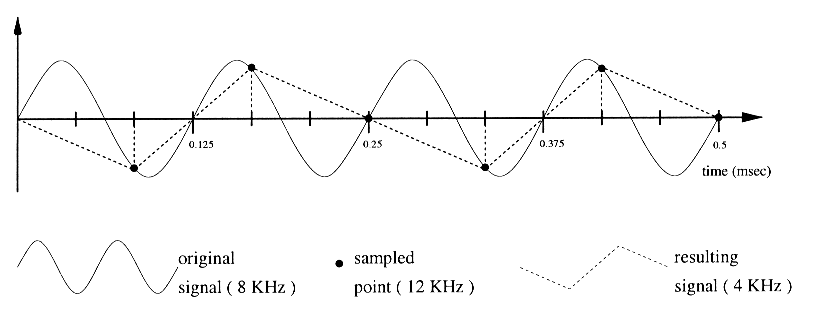
\includegraphics[width=0.8\linewidth]{nyquist}
        \end{center}

    \item \eg if sound signal changes at 3kHz, you have to sample at at least
        6kHz to not miss anything of the signal.
\end{itemize}

\end{frame}

\begin{frame}{Nyquist: example}

    \begin{center}

        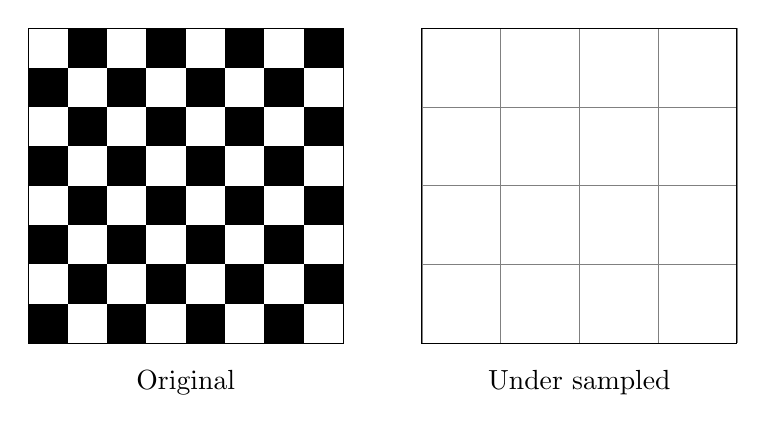
\begin{tikzpicture}[rectangle/.style={fill=black}]

            \node at (-2,-0.5) [anchor=center] {Original};
            \node at (3,-0.5) [anchor=center] {Under sampled};
            \foreach \x in {-4,...,-1} {
                \foreach \y in {0,...,3} {
                    \fill (\x,\y) rectangle (\x+0.5,\y+0.5);
                    \fill (\x+0.5,\y+0.5) rectangle (\x+1,\y+1);
                }
            }
            \draw[help lines] (1,0) grid (5,4);
            \draw (-4,0) rectangle (0,4);
            \draw (1,0) rectangle (5,4);

        \end{tikzpicture}
    \end{center}
Under sampling results in \emph{aliasing} (in computer imaging this is
tackled by anti-aliasing).

\end{frame}

\begin{frame}{Characterizing Error in Mobile Robotics}
    \begin{itemize}
        \item Mobile Robot has to perceive, analyze and interpret the state of the
            surrounding

        \item Measurements in real world environment are dynamically changing and
            error prone.

        \item Examples:

            \begin{itemize}
                \item  changing illuminations

                \item specular reflections

                \item light or sound absorbing surfaces

                \item cross-sensitivity of robot sensor to robot pose and robot-environment
                    dynamics

                    \begin{itemize}

                        \item
                            rarely possible to model \rightarrow appear as random errors
                        \item
                            systematic errors and random errors might be well defined in
                            controlled environment.\\\emph{This is not the case for mobile robots
                            !!}
                    \end{itemize}

            \end{itemize}
    \end{itemize}
\end{frame}

\begin{frame}{Multi-Modal Error Distributions: The Challenges in
    \ldots{}}

    Behavior of sensors modeled by probability distribution (random errors)

    \begin{itemize}
        \item usually very little knowledge about the causes of random errors

        \item often probability distribution is assumed to be symmetric or even
            Gaussian

        \item however, it is important to realize how wrong this can be!

        \item Examples:
            \begin{itemize}
                \item Sonar (ultrasonic) sensor might overestimate the distance in real
                    environment and is therefore not symmetric.
                            \footnotesize Thus the sonar sensor might be best modeled by two
                            modes:

                    \begin{itemize}

                        \item mode for
                            the case that the signal returns directly 
                        \item mode for the case that the
                            signals returns after multi-path reflections.
                    \end{itemize}

                \item Stereo vision system might correlate to images incorrectly, thus causing
                    results that make no sense at all.
            \end{itemize}

    \end{itemize}
\end{frame}

%%%%%%%%%%%%%%%%%%%%%%%%%%%%%%%%%%%%%%%%%%%%%%%%%%%%%%%%%%%%%%%%%%%%%%%%%%
%%%%%%%%%%%%%%%%%%%%%%%%%%%%%%%%%%%%%%%%%%%%%%%%%%%%%%%%%%%%%%%%%%%%%%%%%
\section[Sensors Overview]{Overview of sensors often used on mobile robots}


\begin{frame}{Wheel / Motor Encoders}

\begin{itemize}
    \item Measures position or speed of the wheels or steering.

\item Wheel movements can be integrated to get an estimate of the robots
position \rightarrow odometry.

\item Optical encoders are proprioceptive sensors

\begin{itemize}

\item
  Due to errors (slippage etc.) the position estimate in relation to a
  fixed reference frame is only valuable for short movements.
\end{itemize}

\item Typical resolutions: 2000 increments per revolution.

\begin{itemize}

\item
  For high resolution: interpolation.
\end{itemize}

\item Quadrature encoder (two emittor/detector pairs)

\begin{itemize}

\item
  Gives direction and 4 times higher resolution.
\end{itemize}

\end{itemize}

    \begin{center}
        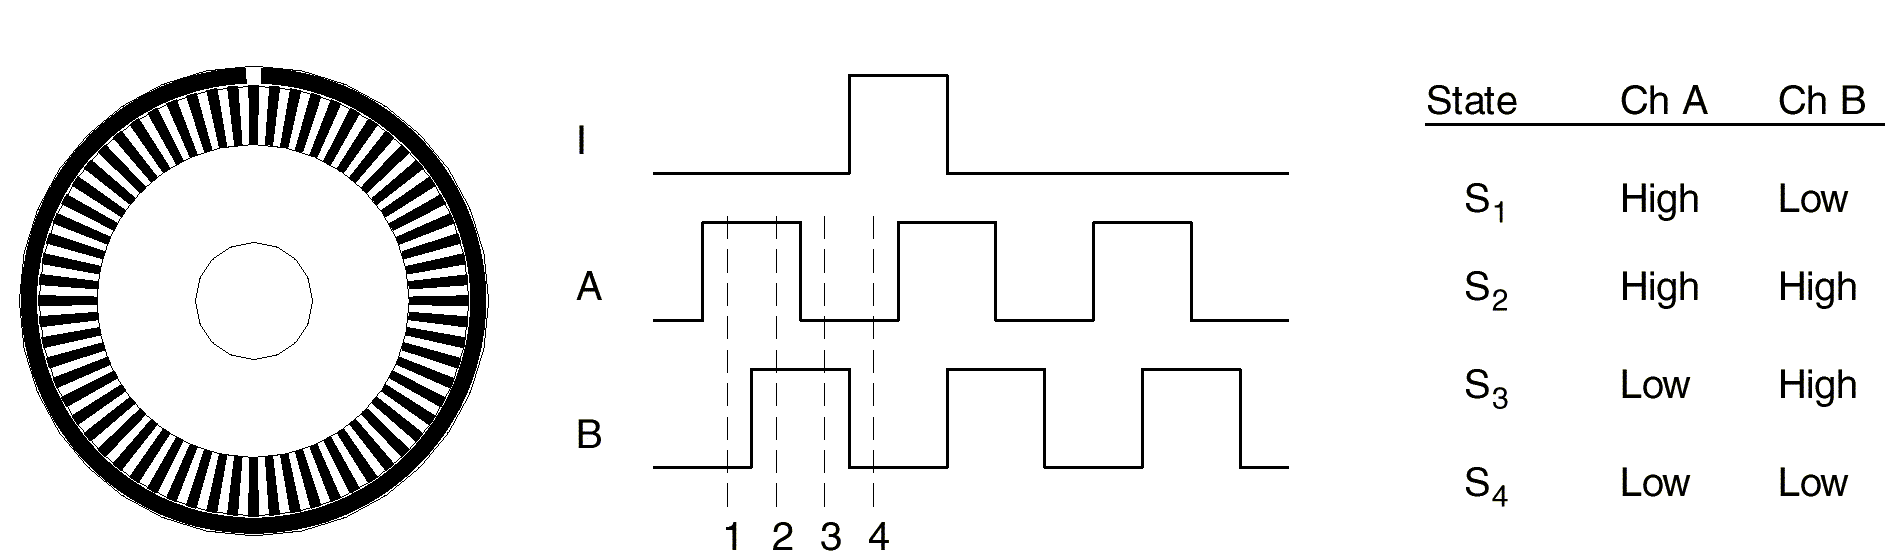
\includegraphics[width=0.9\linewidth]{encoders1}
    \end{center}

\end{frame}

\begin{frame}{Wheel / Motor Encoders}
    \centering

        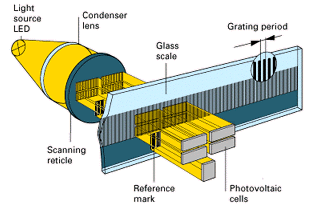
\includegraphics[width=0.45\columnwidth]{encoders2}
        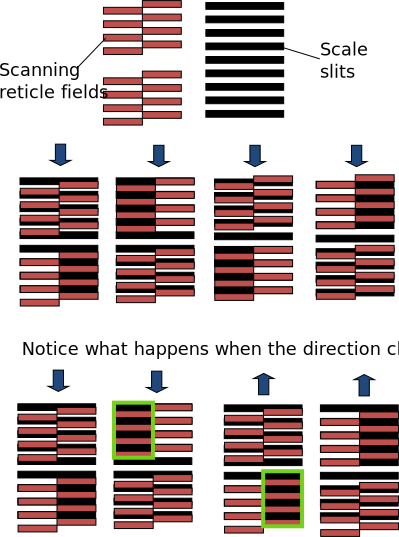
\includegraphics[width=0.45\columnwidth]{encoders}



\end{frame}

\begin{frame}{Wheel / motor encoders}

    \centering
    \begin{multicols}{2}
        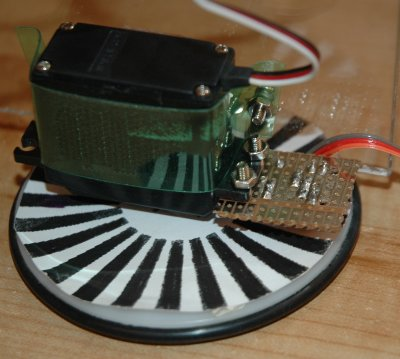
\includegraphics[width=0.6\linewidth]{encoders3}

        Home-made encoder

        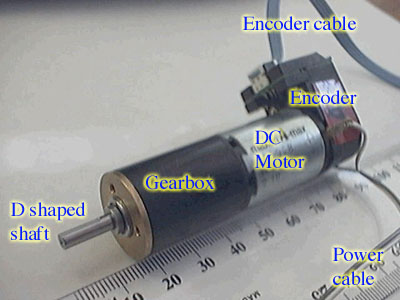
\includegraphics[width=0.6\linewidth]{encoders5}

        Commercial encoder

        \begin{center}
            
\includegraphics[width=0.9\linewidth]{encoders4}
        \end{center}

        Absolute encoder disk

    \end{multicols}

\end{frame}

\begin{frame}{Heading sensors}

    \begin{itemize}
        \item Heading sensors can be proprioceptive (gyroscope, inclinometer) or
            exteroceptive (compass).

        \item Used to determine the robots orientation and inclination.

        \item Allow, together with an appropriate velocity information, to integrate the
            movement to an position estimate. This {\bf odometry} procedure is called
            {\bf dead reckoning} (from ship navigation).

    \end{itemize}
\end{frame}

\begin{frame}{Compass}

Since over 2000 B.C.

\begin{itemize}

\item
  when Chinese suspended a piece of naturally magnetite from a silk
  thread and used it to guide a chariot over land.
\end{itemize}

Magnetic field on earth

\begin{itemize}

\item
  absolute measure for orientation.
\end{itemize}

Large variety of solutions to measure the earth magnetic field

\begin{itemize}

\item
  mechanical magnetic compass
\item
  direct measure of the magnetic field (Hall-effect, magnetoresistive
  sensors)
\end{itemize}

Major drawback

\begin{itemize}

\item
  weakness of the earth field
\item
  easily disturbed by magnetic objects or other sources
\item
  not feasible for indoor environments
\end{itemize}

\end{frame}

\begin{frame}{Compass}

\begin{itemize}

\item
  Solid state compass, \eg Honeywell HMR3100
\end{itemize}

\url{http://datasheet.digchip.com/197/197-01540-0-HMR3100.pdf}

\end{frame}

\begin{frame}{Gyroscope}

Reports an acceleration of rotation to a relative frame of reference.

\begin{itemize}

\item
  Unlike a compass, that keep the orientation to a fixed frame, that
  keeps a reference to an absolute frame of reference.
\end{itemize}

Two categories, the mechanical and the optical gyroscopes

Mechanical Gyroscopes

\begin{itemize}

\item
  Standard gyro
\item
  Rated gyro
\end{itemize}

Optical Gyroscopes

\begin{itemize}

\item
  Rated gyro
\end{itemize}

\end{frame}

\begin{frame}{Mechanical gyroscopes}

Concept: inertial properties of a fast spinning rotor.

\begin{itemize}

\item
  \emph{gyroscopic precession.}
\end{itemize}

Angular momentum associated with a spinning wheel keeps the axis of the
gyroscope inertially stable.

Reactive torque \emph{τ} (tracking stability) is proportional to the
spinning speed \emph{ω}, the precession speed \emph{Ω} and the wheels
inertia \emph{I}.

No torque can be transmitted from the outer pivot to the wheel axis

\begin{itemize}

\item
  spinning axis will therefore be space-stable
\end{itemize}

Quality: 0.1° in 6 hours

If the spinning axis is aligned with the north-south meridian, the
earth's rotation has no effect on the gyro's horizontal axis

\end{frame}

\begin{frame}{If it points east-west, the horizontal axis reads the
earth rotation}

Mechanical gyroscope of ballistic missile (French IRBM S3, 1970s, from
Wikimedia)

\end{frame}

\begin{frame}{Rate gyros}

Same basic arrangement shown as regular mechanical gyros

But: gimble(s) are restrained by a torsional spring

\begin{itemize}

\item
  enables to measure angular speeds instead of the orientation.
\end{itemize}

\end{frame}

\begin{frame}{Optical gyroscopes}

First commercial use started only in the early 1980 when they where
first installed in airplanes.

Optical gyroscopes sensitive to only one plane. Report angular speed
instead of absolute orientation.

One is traveling in a fiber clockwise, the other counterclockwise around
a cylinder (older setups use a ring of mirrors). Based on Sagnac effect.

Laser beam traveling in direction of rotation

\begin{itemize}

\item
  slightly shorter path \rightarrow shows a higher frequency
\item
  difference in frequency Df of the two beams is proportional to the
  angular velocity W of the cylinder
\end{itemize}

Hitachi fibre optical gyroscope

\end{frame}

\begin{frame}{Optical gyros: Sagnac effect}

\begin{itemize}

\item
  A beam of light is split, both beams follow a trajectory in opposite
  directions.
\item
  On return to the point of entry both beams form an interference
  pattern.
\item
  Rotating the apparatus results in a changing interference pattern.
\end{itemize}

\end{frame}

\begin{frame}{Vibrating structure gyroscopes}

A small vibrating element replaces the spinning wheel.

\begin{itemize}

\item
  Measures angular acceleration (= rate gyroscope).
\end{itemize}

Small due to MEMS technology (Micro Electro Mechanical System)

\begin{itemize}

\item
  Lithographic etching of mechanical structure of mm (or smaller) size.
\end{itemize}

Many different ways of implementing this

\begin{itemize}

\item
  Vibrating wheel gyroscope.
\item
  \href{http://en.wikipedia.org/wiki/Piezoelectric_effect}{Piezoelectric}
  element gyroscope.
\item
  Tuning forks manufactured using MEMS technology.
\item
  \ldots{}
\end{itemize}

\end{frame}

\begin{frame}{Technology: vibrating wheel}

Vibrating wheel gyroscope

\begin{itemize}

\item
  Relies on gyroscopic effect, but executed in MEMS technology.
\end{itemize}

Wheel vibrates (equivalent to rotating), tilt due to gyropscopic effect
when, change detected by chance in capacitance.

(from
\href{https://www.quora.com/How-does-a-MEMS-gyroscope-work}{Quora})

\end{frame}

\begin{frame}{Technology: Coriolis effect}

\begin{itemize}

\item
  Mass moving in one direction at speed v, when rotated at speed
  experiences a Coriolis force
\item
  Displacement measured as change in capacitance.
\end{itemize}

\begin{itemize}

\item
  ~
\end{itemize}

(From
\href{http://electroiq.com/blog/2010/11/introduction-to-mems-gyroscopes/}{STM})

\end{frame}

\begin{frame}{Example}

STMicroElectronics

\begin{itemize}

\item
  low-power three-axis angular rate sensor
\item
  I2C, SPI
\item
  70 mdps sensitivity
\item
  \href{http://www.st.com/web/en/resource/technical/document/datasheet/CD00265057.pdf}{Datasheet}
\end{itemize}

In depth information on gyroscopes see
\url{http://ieee-sensors2013.org/sites/ieee-sensors2013.org/files/Serrano_Slides_Gyros2.pdf}

\end{frame}

\begin{frame}{Use of gyroscopes (1)}

Most gyroscopes return angular velocity {[}rad/s{]}

\begin{itemize}

\item
  Angular velocity can be converted to angle (``attitude'' of the gyro)
  through integrating readings over time:
\end{itemize}

While classic optical or mechanical gyroscopes do not suffer from drift,
MEMS gyroscopes do.

\begin{itemize}

\item
  Example, 30º drift over 12 seconds!!
\end{itemize}

(source
\href{http://tom.pycke.be/mav/70/gyroscope-to-roll-pitch-and-yaw}{Tom
Pycke})

Just so know: a variable with a dot on top is that variable at a
particular moment in time\ldots{}

\end{frame}

\begin{frame}{Use of gyroscopes (2)}

\href{http://en.wikipedia.org/wiki/Microelectromechanical_systems}{MEMS}
gyroscopes are very noisy

Filtering needed to get rid of noise.

\begin{itemize}

\item
  Runge-Kutta filter, implements a ``running average'', smoothing out
  the noise.
\end{itemize}

\begin{itemize}

\item
  ~
\end{itemize}

(source
\href{http://tom.pycke.be/mav/70/gyroscope-to-roll-pitch-and-yaw}{Tom
Pycke})

Gyro rotates 90º clockwise and then 90º counter clockwise and back.

Blue line is raw output from gyro, red is low pass filtered.

\end{frame}

\begin{frame}{Accelerometers}

Accelerometers measure acceleration of the device

\begin{itemize}

\item
  Single axis: only measure a in one direction.
\item
  Multi axis: measures in multiple direction, 3 axis is sufficient.
\item
  Measured in m/s2 or in g = 9.81 m/s2.
\end{itemize}

Principle: a damped mass on a spring, when mass accelerates,
displacement is measured and translated to acceleration.

\begin{itemize}

\item
  Modern accelerometers are \emph{micro electro- mechanical
  systems}~(\href{http://en.wikipedia.org/wiki/Microelectromechanical_systems}{MEMS}).
\item
  Displacement is often indirectly measured using capacitive,
  peizoelectric or
  \href{http://en.wikipedia.org/wiki/Piezoresistive_effect}{piezoresistive}
  sensors.
\end{itemize}

Crystalline material changes resistance when under pressure

(\href{http://research.et.byu.edu/llhwww/intro/memsintro.html}{BYU})

\end{frame}

\begin{frame}{Accelerometer as tilt sensor}

An accelerometer always senses the Earth's gravitational vector
(\emph{g} = 9.81 m/s2).

As such an accelerometer can be used to measure rotation.

\begin{itemize}

\item
  However, it cannot measure rotation around the z-axis, for that a
  gyroscope is still needed.
\item
  Gravity vector will be sensed on all three axes as \emph{gx, gy, gz}.
\item
  The gravitation vector can be decomposed in three components, which
  need to vector sum to \emph{g}.
\end{itemize}

\emph{z}

\emph{y}

\emph{x}

\emph{g=}9.81\emph{m/s2}

\emph{z}

\emph{y}

\emph{x}

\emph{g=}9.81\emph{m/s2}

\emph{gz}

\emph{gx}

\emph{gy}

\end{frame}

\begin{frame}{Global Positioning System (GPS)}

\begin{itemize}

\item
  Developed for military use (since 1978).
\item
  Cost of maintenance estimated at \$400M per year.
\item
  Recently it became accessible for commercial applications
\item
  24 satellites (excluding five spares) orbit the earth every 12 hours
  at a height of 20,190 km.
\item
  4 satellites are located in each of six planes inclined 55 degrees
  with respect to the plane of the earth's equators.
\item
  From any location on the planet at least 4 satellites can be seen.
\end{itemize}

\end{frame}

\begin{frame}{Position of satellites}

\begin{itemize}

\item
  Earth diameter ≈ 12,756km, height of GPS satellites ≈ 20,190km.
\item
  From \url{http://www.kowoma.de/en/gps/orbits.htm}
\end{itemize}

\end{frame}

\begin{frame}{GPS - summary}

\begin{itemize}

\item
  Location of any GPS receiver is determined through a time of flight
  measurement.
\item
  Two forms of clock information: Coarse / Acquisition code which is
  public and Precise code which is for military apps. The code also
  carries the identifier of the satellite.
\item
  Satellites carry high-precision atomic clocks, while GPS receivers
  have low precision crystal oscillator clocks (updated by the atomic
  clocks).
\end{itemize}

\end{frame}

\begin{frame}{GPS -- calculating position}

\begin{itemize}

\item
  Suppose the time of flight to three satellites is known: \emph{t1, t2,
  t3}.
\item
  The distance to each satellite is
\item
  If the receivers position is \emph{(x,y,z)}, and the satellites
  position is \emph{(x1, y1, z1)}, \emph{(x2, y2, z2)} and \emph{(x3,
  y3, z3)}, the following relations hold
\end{itemize}

\end{frame}

\begin{frame}{GPS -- calculating position}

Three spheres, intersection results in two solutions for \emph{(x,y,z)}.
One is above the earth's surface, the other below.

A deviation in the receivers clock, results a error on the distance to
the satellite.

\begin{itemize}

\item
  For example, satellite at 25,000km from receiver, 0.1ms deviation
  between clocks, results in an error of 30m in the distance to the
  satellite.
\end{itemize}

\end{frame}

\begin{frame}{GPS -- calculating position}

\begin{itemize}

\item
  Assume time difference between atomic clocks and receiver clock is
  Δ\emph{t}. The distance to the satellites is now erroneously estimated
  at
\item
  Δ\emph{t} can be calculated by taking an extra satellite into account.
\end{itemize}

\end{frame}

\begin{frame}{GPS - accuracy}

With the C/A code, the time of flight can be measured to within 10ns,
which is an error of ≈ 3m.

Sources of error on the distance to satellite estimate

\begin{itemize}

\item
  Ionospheric effects: ± 5 meter
\item
  Ephemeris errors: ± 2.5 meter
\item
  Satellite clock errors: ± 2 meter
\item
  Multipath distortion: ± 1 meter
\item
  Tropospheric effects: ± 0.5 meter
\item
  Numerical errors± 1 meter or less
\end{itemize}

Typical accuracy is 15 m, but this varies a lot.

\end{frame}

\begin{frame}{GPS - improvements}

L1 and L2 frequency.

\begin{itemize}

\item
  Same time information is transmitted on two frequencies, these
  frequencies will experience noise in a different way. Can be used to
  cancel noise.
\end{itemize}

Differential GPS (DGPS)

\begin{itemize}

\item
  Stationary receiver, with known position, read GPS position and
  calculate the error. This error is broadcast over an FM band to
  receiver in the neighbourhood. Accuracy is 1 to 3 meters.
\end{itemize}

Satellite Based Augmentation System (SBAS)

\begin{itemize}

\item
  Ground based receivers calculate ionospheric delays and clock drift,
  this is relayed to geosynchronous satellites which then broadcast it
  to all receivers in its view.
\item
  The American Federal Aviation Administration~ has a system which works
  in the Western hemisphere, called Wide Area Augmentation
  System~(WAAS)~.
\end{itemize}

\end{frame}

\begin{frame}{Galileo}

Europe's response to GPS (or GLONASS, the Russian global positioning
system).

\begin{itemize}

\item
  30 spacecraft
\item
  orbital altitude: 23,222 km
\item
  3 orbital planes, 56° inclination (9 operational satellites and one
  active spare per orbital plane)
\item
  satellite lifetime: \textgreater{}12 years
\end{itemize}

Better

\begin{itemize}

\item
  Free access: 1m accuracy.
\item
  Subscription access: up to 10cm accuracy.
\item
  Better high altitude positioning.
\end{itemize}

\end{frame}

\begin{frame}{GPS - Receivers}

\textbf{SparkFun - 20 channel EM-406A SIRF III receiver}

\begin{itemize}

\item
  16g including cable
\item
  20-Channel Receiver
\item
  Extremely high sensitivity : -159dBm
\item
  10m Positional Accuracy / 5m with WAAS
\item
  Hot Start : 8s
\item
  Cold Start : 42s
\item
  70mA at 4.5-6.5V
\item
  Outputs NMEA 0183 and SiRF binary protocol
\item
  Smallest complete module available: 30mm x 30mm x 10.5mm
\item
  £43.80 (in 2008)
\end{itemize}

\textbf{Sparkfun 54 Channel USB stick receiver}

\begin{itemize}

\item
  \$80 (in 2008)
\end{itemize}

\end{frame}

\begin{frame}{GPS -- Applications in robotics}

GPS only works \textbf{outdoors}

\begin{itemize}

\item
  Due to limited energy (--163 dBw~or 5 x 10--17~watts) and high
  frequency (1.57542~GHz for L1 signal and 1.2276~GHz for L2 signal) of
  signal, GPS packets do not penetrate buildings.
\end{itemize}

Limited accuracy when relying on GPS and DGPS

\begin{itemize}

\item
  Accuracy several meters up to tens of meters. Autonomous vehicles will
  need to rely on other localisation methods.
\end{itemize}

Accuracy can be dramatically improved using a local DGPS antenna.

\begin{itemize}

\item
  \url{http://www.racelogic.co.uk/}
\end{itemize}

\url{http://www.youtube.com/watch?v=FATVNEB1_BY}

\end{frame}

\begin{frame}{Examples}

\begin{itemize}

\item
  Positioning of outdoor service robots:
  \href{http://www.robotera.eu/}{www.robotera.eu}
\end{itemize}

Agricultural robots

\begin{itemize}

\item
  Sowing, weeding, harvesting with cm precision
\end{itemize}

\end{frame}

\begin{frame}{Other localisation methods}

Mainly used in mobile phones and mobile devices.

GSM base triangulation.

\begin{itemize}

\item
  Uses strength of GSM signal of different GSM base stations to estimate
  position.
\item
  Works indoors, but accuracy limited to a radius of about 1km.
\end{itemize}

WiFi based localisation.

\begin{itemize}

\item
  If a device connects to a WiFi router, it knows the IP address of the
  router. Some internet providers know at which address a router is and
  provide this.
\item
  Google Gears supports this service.
\item
  More accurate as range of WiFi router is limited, radius of about 50m.
  But not all IP provide network locations.
\end{itemize}

\end{frame}

\begin{frame}{Range sensors (time of flight)}

Large range distance measurement \rightarrow called range sensors

Range information:

\begin{itemize}

\item
  key element for localization and environment modeling
\end{itemize}

Ultrasonic sensors as well as laser range sensors make use of
propagation speed of sound or electromagnetic waves respectively. The
traveled distance of a sound or electromagnetic wave is given by \emph{d
= c . t}

Where

\begin{itemize}

\item
  d = distance traveled (usually round-trip)
\item
  c = speed of wave propagation
\item
  t = time of flight.
\end{itemize}

\end{frame}

\begin{frame}{Range sensors (time of flight)}

It is important to point out

Propagation speed \emph{v} of sound: 0.3 m/ms

Propagation speed \emph{v} of of electromagnetic signals: 0.3 m/ns,

\begin{itemize}

\item
  one million times faster.
\end{itemize}

3 meters

\begin{itemize}

\item
  is 10 ms ultrasonic system
\item
  only 10 ns for a laser range sensor
\item
  time of flight t with electromagnetic signals is not an easy task
\item
  laser range sensors expensive and delicate
\end{itemize}

The quality of time of flight range sensors mainly depends on:

\begin{itemize}

\item
  Uncertainties about the exact time of arrival of the reflected signal,
  due to reflections, multiple echo's, \ldots{}
\item
  Internal sensor inaccuracies in the time of flight measure (laser
  range sensors)
\item
  Opening angle of transmitted beam (ultrasonic range sensors)
\item
  Interaction with the target (surface, specular reflections)
\item
  Variation of propagation speed
\item
  Speed of mobile robot and target (if not at standing still)
\end{itemize}

\end{frame}

\begin{frame}{Ultrasonic Sensor (sonar)}

\begin{itemize}

\item
  Transmit a packet of (ultrasonic) pressure waves.
\item
  Distance d of the echoing object can be calculated based on the
  propagation speed of sound \emph{c} and the time of flight \emph{t}.
\item
  The speed of sound \emph{c}gas in a gas is given by
\end{itemize}

\end{frame}

\begin{frame}{Speed of sound in air}

Can be approximated by with the air temperature in Celcius.

If no correction for temperature would be done, what would the error be?

\begin{itemize}

\item
  Assume obstacle at 1m, and T = 15°C.
\end{itemize}

\end{frame}

\begin{frame}{Signals of ultrasonic sensor}

Transmitted sound

Analog echo signal

threshold

Digital echo signal

Integrated time

Output signal

integrator

Time of flight (sensor output)

threshold

Wave packet

\end{frame}

\begin{frame}{Ultrasonic sensor properties}

Typically a frequency: 40 - 180 kHz

Generation of sound wave: piezo transducer

\begin{itemize}

\item
  transmitter and receiver separated or not separated.
\end{itemize}

Sound beam propagates in a cone like manner

\begin{itemize}

\item
  opening angles around 20 to 40 degrees
\item
  regions of constant depth
\item
  segments of an arc (sphere for 3D)
\end{itemize}

\end{frame}

\begin{frame}{Problems with reflection}

\begin{itemize}

\item
  Soft surfaces absorb most of the acoustic energy.
\item
  Surfaces that are fare from being perpendicular to the direction of
  the sound: specular reflection.
\end{itemize}

a) 360° scan

b) results from different geometric primitives

\end{frame}

\begin{frame}{Cycle time of ultrasonic sensors}

When emitter and receiver are one and the same piece of hardware, the
sensor has a \emph{blanking time}.

\begin{itemize}

\item
  Time after the ping in which the sensor is blind.
\item
  Close obstacles will be missed.
\end{itemize}

Cycle time is rather low.

\begin{itemize}

\item
  In a moderately sized room where obstacles are 3m away, the time of
  flight is about 20ms. The sensor refresh rate is 50Hz.
\item
  However, if a ring of sonar sensors is used, only one sensor at a time
  can be fired. For example, a 20 sensor ring will only operate at
  2.5Hz.
\end{itemize}

\end{frame}

\begin{frame}{Sonar sensors}

LV-MaxSonar

\begin{itemize}

\item
  \url{http://www.maxbotix.com/}
\item
  Detect 0 to 6.5m, range sensing 0.2 to 6.5m
\item
  42 kHz sonar ping.
\item
  Serial out.
\item
  Free run or triggered.
\item
  \$25 - \$30 (in 2008).
\end{itemize}

\end{frame}

\begin{frame}{Laser Range Sensor}

Transmitted and received beams coaxial.

Transmitter illuminates a target with a collimated beam.

Receiver detects the time needed for round-trip.

A mechanical mechanism with a mirror sweeps

\begin{itemize}

\item
  2 or 3D measurement
\end{itemize}

Parallel rays of electromagnetic energy

Diffuse reflection, resulting in near isotropic reflection.

\end{frame}

\begin{frame}{Measuring time of flight of light}

Pulsed laser.

\begin{itemize}

\item
  measurement of elapsed time directly.
\item
  resolving picoseconds \rightarrow expensive hardware.
\end{itemize}

Indirectly: the time of flight can be measured using a phase shift
measurement to produce range estimation.

\begin{itemize}

\item
  technically easier than the above two methods.
\end{itemize}

\end{frame}

\begin{frame}{Phase-shift measurement of TOF}

Phase-shift Measurement

\end{frame}

\begin{frame}{****}

\end{frame}

\begin{frame}{Where \emph{c}: is the speed of light; \emph{f} the
modulating frequency; \emph{D'} covered by the emitted light is,
\emph{θ} is phase shift.}

\begin{itemize}

\item
  for f = 5 Mhz (as in the AT\&T sensor), l = 60 meters
\end{itemize}

l = \emph{c/f}

Θ in radians, θ/2π is {[}0..1{]}

\end{frame}

\begin{frame}{Phase-shift measurement of TOF}

Distance D, between the beam splitter and the target where  phase
difference between the transmitted and received beam.

Theoretically ambiguous range estimates

\begin{itemize}

\item
  since for example if  = 60 meters, a target at a range of 5 meters =
  target at 35 meters
\end{itemize}

\end{frame}

\begin{frame}{Example}

Laser range scanners in outdoor robotics application point down.

\begin{itemize}

\item
  If they would look at the horizon, they would return ambiguous
  measurements.
\end{itemize}

\end{frame}

\begin{frame}{Other practical issues}

Confidence in the range (phase estimate) is inversely proportional to
the square of the received signal amplitude.

\begin{itemize}

\item
  Hence dark, distant objects will not produce such good range estimated
  as closer brighter objects \ldots{}
\end{itemize}

\end{frame}

\begin{frame}{2D laser range scanner}

\begin{itemize}

\item
  Typical range image of a 2D laser range sensor with a rotating mirror.
  The length of the lines through the measurement points indicate the
  uncertainties.
\end{itemize}

\end{frame}

\begin{frame}{Laser range finder}

Hokuyo URG-04LX

\begin{itemize}

\item
  240° field of view.
\item
  0.36° angular resolution.
\item
  10 Hz scan rate.
\item
  USB (and RS232) interface.
\item
  Range 20mm to 4m.
\item
  Dimensions 50 x 50 x 71mm
\item
  £900 (in 2010, down from £1800 in 2008).
\end{itemize}

\url{http://www.acroname.com/robotics/parts/R283-HOKUYO-LASER1.html}

\end{frame}

\begin{frame}{Triangulation ranging}

Geometrical properties of the image to establish a distance measurement.

Project a well defined light pattern (\eg point, line) onto the
environment.

\begin{itemize}

\item
  reflected light is then captured by a photo-sensitive line or matrix
  sensor device (camera).
\item
  simple triangulation allows to establish a distance.
\end{itemize}

Size of an captured object can be known.

\end{frame}

\begin{frame}{Triangulating distance sensor}

\emph{Target}

\emph{D}

\emph{L}

\emph{Laser / Collimated beam}

\emph{Transmitted Beam}

\emph{Reflected Beam}

\emph{P}

\emph{Position-Sensitive Device (PSD)}

\emph{or Linear Camera}

\emph{x}

\emph{Lens}

Principle of 1D laser triangulation.

\begin{itemize}

\item
  distance is proportional to the 1/x
\end{itemize}

\end{frame}

\begin{frame}{Sharp GP series distance sensors}

\begin{itemize}

\item
  Cheap (≈ £6).
\item
  Distance measurement between 8 and 80cm (for GP2D12 model).
\item
  Output: analogue voltage.
\item
  Less dependant on reflectivity of material than normal IR distance
  sensors.
\item
  Measurement every 40ms.
\end{itemize}

\end{frame}

\begin{frame}{Structured light (vision, 2D, 3D)}

\begin{itemize}

\item
  Eliminate the correspondence problem of stereo vision by projecting
  structured light on the scene.
\item
  Project slits of light or emits collimated light (\eg laser) by means
  of a rotating mirror.
\item
  Reflection sensed by camera.
\item
  Range to an illuminated point can be determined from simple geometry.
\end{itemize}

\end{frame}

\begin{frame}{Structured light (vision, 2D, 3D)}

\emph{b}

\emph{u}

\end{frame}

\begin{frame}{Structured light -- 1D illustration}

\begin{itemize}

\item
  One dimensional schematic of the principle
\item
  From the figure, simple geometry shows that:
\end{itemize}

\end{frame}

\begin{frame}{Structured light -- 1D illustration}

Range resolution is defined as the triangulation gain \emph{Gp.}

Baseline length \emph{b}

\begin{itemize}

\item
  the smaller \textbf{\emph{b}} is the more compact the sensor can be.
\item
  the larger \emph{b} is the better the range resolution is.
\end{itemize}

Focal length \emph{f}

larger focal length \emph{f} gives

\begin{itemize}

\item
  a smaller field of view
\item
  an improved range resolution
\item
  less lens distortion
\end{itemize}

however, large focal length means a larger sensor head.

\end{frame}

\begin{frame}{Camera}

Hardware

Two technologies: CCD or CMOS.

Monochrome or colour.

Resolution between 1 x 64 pixels and 4000 x 4000 pixels.

Small, low-power and cheap.

Prices anything between 40p and £3000.

\begin{itemize}

\item
  Cameras have dropped significantly in price, and are the cheapest
  high-tech sensor around.
\end{itemize}

\end{frame}

\begin{frame}{Camera output}

Most cameras provide digital output.

\begin{itemize}

\item
  USB1.0, USB1.1, USB2.0, Firewire (aka IEEE 1394 or i.Link, ethernet),
  or any hardware bus or proprietary bus.
\end{itemize}

Some --mostly older- camera designs do not, and provide an analog (RGB
or composite) signal instead.

\begin{itemize}

\item
  A \textbf{frame grabber} is needed to digitise the signal.
\item
  Matrox the leading manufacturer of frame grabbers.
\end{itemize}

\end{frame}

\begin{frame}{Camera parameters}

Shutter speed

\begin{itemize}

\item
  Rate at which an image is refreshed, \eg 25ms, 1/400 s.
\end{itemize}

Iris position (aka aperture)

\begin{itemize}

\item
  Size of the lens opening, mechanically operated. Allows more or less
  light in.
\end{itemize}

Camera gain

\begin{itemize}

\item
  Amplification of the camera signal. \textbf{Noise is amplified as
  well.}
\end{itemize}

White balance (aka color temperature)

\begin{itemize}

\item
  Mixture of blue, red and green components that define white. Often
  needed to cancel out influences of illumination.
\end{itemize}

\end{frame}

\begin{frame}{CCD technology}

Charge-coupled device (CCD).

\begin{itemize}

\item
  Each pixel has a photodiode and a capacitor, the capacitor is charged
  or discharged as photons hit the light-sensitive silicon.
\item
  The charge in the capacitor is proportional to the light intensity.
\item
  The charge is read out at the corner of the chip's surface.
\item
  Charge is transferred over the chip' surface to that corner, like a
  ``bucket brigade''.
\end{itemize}

\end{frame}

\begin{frame}{CCD technology}

Some sort of shutter is needed to prevent smear in the camera image.

\begin{itemize}

\item
  Mechanical shutter: expensive and high power consumption.
\item
  Frame transfer CCD: one half of the chip's surface is opaque, charge
  is transferred there and then read out.
\item
  Interline architecture: every other line is opaque, faster shutter
  speeds possible. Less sensitive to light.
\end{itemize}

\end{frame}

\begin{frame}{CCD technology}

Sensitive to wavelengths 400nm to 1000nm.

\begin{itemize}

\item
  Human visual spectrum from 380nm to 780nm, so less sensitive to blue
  light and oversensitive to red and \textbf{infrared}.
\end{itemize}

\end{frame}

\begin{frame}{CCD - advantages}

High quality, relatively low noise images.

High quantum efficiency

\begin{itemize}

\item
  70 to 80\% of photons are converted into a charge, ideal for low light
  conditions.
\end{itemize}

Integrating function of pixels.

\begin{itemize}

\item
  Can be used to measure for prolonged times in very dim settings.
\end{itemize}

\end{frame}

\begin{frame}{CCD- disadvantages}

Large silicon size

\begin{itemize}

\item
  Due to circuitry to read out pixels.
\end{itemize}

Interfacing between CCD and CMOS technology is not straight-forward

\begin{itemize}

\item
  Hinders cheap hardware.
\end{itemize}

Complex clocking issues on chip.

Large dissipation.

Integrating light measurement

\begin{itemize}

\item
  In bright light, capacitors can become saturated. This causes blooming
  the image.
\end{itemize}

\end{frame}

\begin{frame}{CMOS technology}

Complementary metal oxide semiconductor (CMOS)

\begin{itemize}

\item
  Photodiode with circuitry that reads out light intensity.
\item
  \textbf{No} integrating measurement, but a \textbf{proportional}
  measurement instead.
\item
  Pixel values are read out much like in RAM memory.
\end{itemize}

\end{frame}

\begin{frame}{CMOS - advantages}

CMOS technology is mature and simple

\begin{itemize}

\item
  Production costs are a fraction of that of CCD.
\end{itemize}

No complex clocking in chip.

Low power consumption.

Proportional measurement

\begin{itemize}

\item
  No saturation of pixels.
\end{itemize}

Smaller silicon size.

Random access to pixels (just like RAM).

Easy interfacing to CMOS technology.

\begin{itemize}

\item
  CMOS circuitry, \eg for bus, can be integrated on the same silicon
  area.
\end{itemize}

\end{frame}

\begin{frame}{CMOS - disadvantages}

Each photodiode has CMOS circuitry which takes up silicon real estate,
but is not sensitive to incoming light.

\begin{itemize}

\item
  CMOS camera is less sensitive than CCD.
\end{itemize}

CMOS has a larger pixel mismatch and is typically more noisy than CCD.

\begin{itemize}

\item
  This has improved considerably over the years, see CMOS in high-end
  \#\# digital cameras.
\end{itemize}

\end{frame}

\begin{frame}{Colour cameras}

With one CCD or CMOS sensor, a filter is placed in front of the sensor
surface.

\begin{itemize}

\item
  Resolution, relative to monochrome camera, is reduced by 75\%.
\item
  Bayer (GRGB) or RGBE (E = Emerald) filter.
\end{itemize}

Bayer filter

\end{frame}

\begin{frame}{RGBE filter}

\end{frame}

\begin{frame}{Colour cameras}

Three sensor cameras.

\begin{itemize}

\item
  In expensive and professional colour cameras, the images is optically
  split in three.
\item
  Each copy is sent to a separate sensor, each sensor has a R, G, or B
  filter.
\end{itemize}

No resolution loss due to Bayer or RGBE filter.

No problem of misalignment of filter.

\end{frame}

\begin{frame}{Omnidirectional camera}

\begin{itemize}

\item
  Most robots need 360° vision, this can be provided by a
  \textbf{omnidirectional camera}.
\end{itemize}

\end{frame}

\begin{frame}{Image processing and computer vision}

\begin{itemize}

\item
  See Phil Culverhouse's lectures.
\item
  Take an MSc Robotics next year.
\end{itemize}

\end{frame}

\begin{frame}{Depth camera technologies}

Stereo cameras.

3D single lens cameras.

\begin{itemize}

\item
  Swissranger
\item
  Primesense (XBox Kinect)
\end{itemize}

\end{frame}

\begin{frame}{Stereo cameras}

\begin{itemize}

\item
  A camera typically forms a 2D mapping of a 3D environment.
\item
  Reconstructing depth from a 2D image is in most cases impossible.
\item
  A solution to this is using a \textbf{stereo camera} which can
  calculate the depth (i.e.~z axis) of pixels.
\item
  Using two slightly different views from the same scene and a precise
  knowledge of camera parameters.
\end{itemize}

(Videre design, www.videredesign.com)

(JPL)

\end{frame}

\begin{frame}{Stereo cameras (2)}

Each camera gives slightly shifted view of the scene

\begin{itemize}

\item
  Depending on the size of the shift one can determine how far obstacles
  are.
\end{itemize}

The challenge of finding corresponding pixels in the two images.

\begin{itemize}

\item
  It often is very hard to find pixels that correspond in the two
  images.
\end{itemize}

(Wikipedia)

\end{frame}

\begin{frame}{Stereo cameras (3)}

Disadvantages

\begin{itemize}

\item
  Two calibrated cameras needed.
\item
  Multiple computationally intensive steps.
\item
  Depends on illumination and scene texture.
\end{itemize}

More at
\href{http://campar.in.tum.de/twiki/pub/Chair/TeachingSs11Kinect/2011-DSensors_LabCourse_Kinect.pdf}{TUM}

\end{frame}

\begin{frame}{Swissranger 3D camera}

MESA SR3000

\begin{itemize}

\item
  Uses TOF measured as phase difference of IR light.
\item
  CCD camera at 176 x 144 resolution.
\item
  Frame rate, 29fps at 0.3m to 12fps at 3m.
\item
  Accuracy: 3mm (best case).
\item
  \$7500 (in 2008)
\end{itemize}

\end{frame}

\begin{frame}{Microsoft Kinect}

\textbf{Kinect 360} (also known as version 1). Released in 2010.

\textbf{Kinect One} (also known as version 2). Released in 2014.

\end{frame}

\begin{frame}{Kinect 360 - Primesense 3D camera}

Infrared laser light pattern projected onto scene and filmed with CMOS
camera.

\begin{itemize}

\item
  Class 1 laser device: safe for eyes.
\item
  1cm depth resolution, 3mm height and width.
\item
  320x240 16-bit depth @ 30 frames/sec, 640x480 32-bit colour@ 30
  frames/sec, 16-bit audio @ 16 kHz
\item
  Stronger light than Swissranger 3D cam: laser dots vs LED light.
\end{itemize}

\end{frame}

\begin{frame}{Kinect 360 - Primesense 3D camera}

The hardware is only one aspect of the sensor.

The software is equally important.

\begin{itemize}

\item
  Matching a cloud of points in 3D space to 2 body models is a very hard
  problem in artificial intelligence.
\item
  Machine learning used to let the software learn mapping between 3D
  points and body models (see
  \href{http://www.theinstitute.ieee.org/portal/site/tionline/menuitem.130a3558587d56e8fb2275875bac26c8/index.jsp?\&pName=institute_level1_article\&TheCat=2201\&article=tionline/legacy/inst2011/jan11/featuretech.xml\&}{IEEE
  article})
\end{itemize}

\end{frame}

\begin{frame}{Kinect 360 - Primesense 3D camera}

Principles

\begin{itemize}

\item
  Dot pattern (speckles) is projected in near IR light.
\item
  CMOS IR camera records image.
\item
  Pattern is known by sensor. Calibration is done at time of
  manufacturing: a set of calibration images is stored in the device.
\item
  Each dot pattern encodes a coordinate
\end{itemize}

From
\href{http://worldwide.espacenet.com/publicationDetails/originalDocument?FT=D\&date=20100909\&DB=EPODOC\&locale=en_EP\&CC=US\&NR=2010225746A1\&KC=A1}{US
Patent}

\end{frame}

\begin{frame}{Kinect skeleton tracking}

\begin{itemize}

\item
  Reading depth image is only one part what the Kinect does.
\item
  It also infers skeleton (positions of torse, head, arms and legs) from
  depth image.
\item
  Based on machine learning
  (\href{http://research.microsoft.com/pubs/145347/BodyPartRecognition.pdf}{Shotton
  et al., 2011})
\end{itemize}

\end{frame}

\begin{frame}{Machine learning}

100,000 images of people in front of RGBD sensor, together with ``ground
truth'' from a motion capture system.

\begin{itemize}

\item
  Different body types, different clothes.
\end{itemize}

Using machine learning (\emph{randomised decision forest} algorithm) to
find body parts

\begin{itemize}

\item
  A farm of computers required a day to arrive at a solution to separate
  body parts from background images.
\end{itemize}

Microsoft SDK allows tracking of 2 skeleton for Kinect 360 and 5 for
Kinect One.

\end{frame}

\begin{frame}{The Kinect One}

The same, but better!

\begin{itemize}

\item
  Faster full HD video stream
\item
  Better microphones
\item
  Higher depth fidelity
\item
  Wider angle camera (70x60 degrees vs K1 57x43)
\item
  Improved skeleton model (prediction)
\item
  More skeleton points (26)/more people tracked (6 full)
\item
  New development SDK
\item
  More expensive, not as much support as yet
\item
  CANNOT use Xbox version with PC like with v1!
\end{itemize}

\end{frame}

\begin{frame}{360 vs One Technology}

\begin{itemize}

\item
  Kinect 360 project speckle pattern into environment, uses
  triangulation (structured light) from near-IR
\end{itemize}

(WikiMedia)

\end{frame}

\begin{frame}{360 vs One Technology}

Kinect One uses Time-of-Flight (indirectly measured through phase shift
measurements).

Take 2 measurements -- eliminate ambiguity if light is absorbed

Ambient light rejection

\begin{itemize}

\item
  Allows outdoor operation!
\end{itemize}

Excellent explanation
\href{http://www.gamasutra.com/blogs/DanielLau/20131127/205820/The_Science_Behind_Kinects_or_Kinect_10_versus_20.php}{here}

\end{frame}

\begin{frame}{How do we use it?}

2 main options:

\begin{itemize}

\item
  1. Microsoft SDK
\item
  2. OpenNI
\end{itemize}

Microsoft SDK needs specific versions of Visual Studio

Microsoft SDK is best complemented with the Developer Tools (which has
lots of great example applications)

\end{frame}

\begin{frame}{How do we use it? (2)}

Lots of cables -- plug the Kinect into the power adapter, then the USB
to your computer

\begin{itemize}

\item
  Make sure the power is on before you plug it in to a PC, or it will
  see it only as a microphone
\end{itemize}

\end{frame}

\begin{frame}{How do we use it? (3)}

The Microsoft SDK can be programmed with C\#.Net, VB.Net or VC++

\begin{itemize}

\item
  We recommend C\#, but C++ is possible as well
\end{itemize}

Or if you want to try, there are other options as well

\begin{itemize}

\item
  \href{https://processing.org/}{Processing} is a language for
  non-programmers with excellent support for Kinect (see
  \href{http://shiffman.net/p5/kinect/}{here})
\end{itemize}

\end{frame}

\begin{frame}{Programming principles}

\begin{itemize}

\item
  SDK provides interface to find and use sensor in just a few lines
\item
  Events fire when a new RGB frame or depth frame are ready for use, or
  when audio source changes angle or energy
\item
  We put a handler on these events to pick up the images
\item
  We can then read out raw data values, convert images, or use the
  processed data about skeletons/faces
\item
  Continuous audio processing must be done manually in its own thread
\end{itemize}

\end{frame}

\begin{frame}{In robotics applications}

\textbf{Tele-operation:}

\begin{itemize}

\item
  Plymouth: \url{https://www.youtube.com/watch?v=wf4waMhPHmc}
\item
  Plymouth Baxter: \url{https://www.youtube.com/watch?v=XKRI0hcInqE}
\item
  NASA: \url{https://www.youtube.com/watch?v=pqNC72fgetc}
\item
  Full body: \url{https://www.youtube.com/watch?v=7vq-1TiXi3g}
\item
  2 arms: \url{https://www.youtube.com/watch?v=kECNyr7v0kM}
\end{itemize}

Autonomous navigation: \url{https://www.youtube.com/watch?v=eWmVrfjDCyw}

Cutting bananas?:
\url{https://www.youtube.com/watch?v=TmTW61MLm68\#t=356}

\end{frame}


\begin{frame}{}
    \begin{center}
        \Large
        That's all, folk!\\[2em]
        \normalsize
        Questions:\\
        Portland Square A216 or \url{severin.lemaignan@plymouth.ac.uk} \\[1em]

        Slides:\\ \url{github.com/severin-lemaignan/[REPO]}

    \end{center}
\end{frame}



\end{document}
